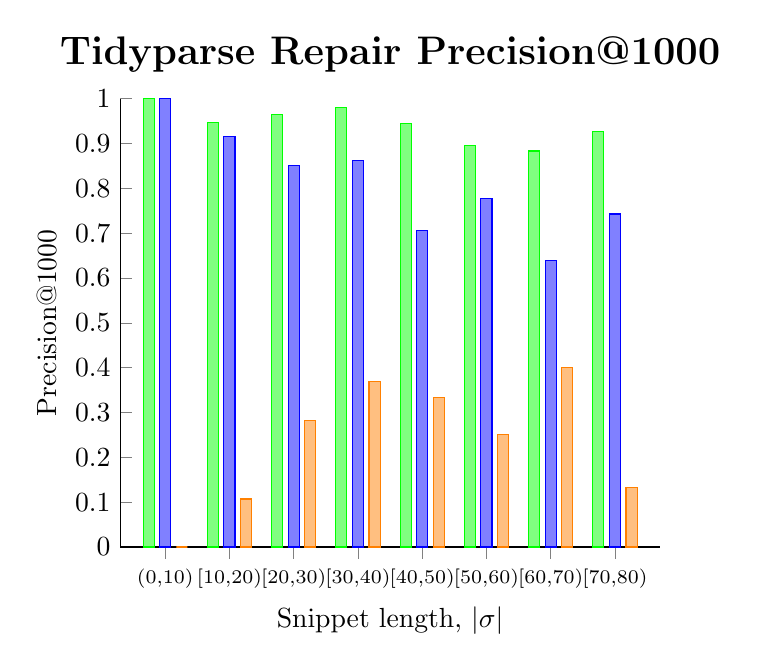
\begin{tikzpicture}
  \begin{axis}[
  xlabel={Snippet length, $|\sigma|$},
  ylabel={Precision@1000},
  title={\Large\textbf{Tidyparse Repair Precision@1000}},
  ybar,
  axis lines*=left,
  xtick={0, 10, 20, 30, 40, 50, 60, 70},
  ytick={0, 0.1, 0.2, 0.3, 0.4, 0.5, 0.6, 0.7, 0.8, 0.9, 1.0},
  xticklabels={{(}0{,}10{)}, {[}10{,}20{)}, {[}20{,}30{)}, {[}30{,}40{)}, {[}40{,}50{)}, {[}50{,}60{)}, {[}60{,}70{)}, {[}70{,}80{)}},
  x tick label style={font=\scriptsize},
  ymax=1.0,
  ymin=0.0,
  bar width=4pt,
  ]
  \addplot[green, fill=green!50] coordinates { (0, 1.0) (10, 0.946236559139785) (20, 0.9641434262948207) (30, 0.9812206572769953) (40, 0.944) (50, 0.8958333333333334) (60, 0.8833333333333333) (70, 0.9264705882352942) };
  \addplot[blue, fill=blue!50] coordinates { (0, 1.0) (10, 0.9157894736842105) (20, 0.8518518518518519) (30, 0.8627450980392157) (40, 0.7066666666666667) (50, 0.7777777777777778) (60, 0.64) (70, 0.7428571428571429) };
  \addplot[orange, fill=orange!50] coordinates { (0, 0.0) (10, 0.10714285714285714) (20, 0.28125) (30, 0.3684210526315789) (40, 0.3333333333333333) (50, 0.25) (60, 0.4) (70, 0.13333333333333333) };
  \end{axis}
\end{tikzpicture}